\chapter{Resultados y análisis}

Aquí se mostrarán los resultados que se obtuvieron con los algoritmos mencionados en la sección anterior. Haciendo un pequeño recuento, los \textit{datasets} usados son archivos que utilizan un formato \textbf{.fasta} y son los siguientes:

\begin{table}[h]
\centering
\begin{tabular}{|l|c|c|c|}
\hline
\multicolumn{1}{|c|}{\textbf{Bases de datos}} & \textbf{Proteínas} & \textbf{Tamaño (MB)} & \textbf{Tamaño cadena (MB)} \\ \hline
SwissProt    & 555.426                & 268,3                & 199,5              \\
TrEMBL        & 89.396.316              & 40.900 (aprox.)       & 30.200 (aprox.)     \\
EROP-Moscow        & 14.785                 & 1,5                  & 0,3526                \\
Proteínas humanas     & 86.298                 & 47,2                 & 38,2               \\ \hline
\end{tabular}
\caption{\textit{Datasets} utilizados para la obtención de resultados}
\label{tb:labelr1}
\end{table} 

\section{Sistema utilizado y método de experimentación}

Los algoritmos se ejecutaron en un servidor Intel(R) Xeon(R) CPU E5-2630 @2.30GHz, cuya memoria RAM posee una capacidad de 60 GB, prestado para la ocasión por la Universidad. Los datos relevantes a esta máquina se aprecian en la \textbf{Tabla 4.2}.

Los programas fueron implementados en C++, mediante el uso del entorno de desarrollo integrado (IDE) ``Code::Blocks'' \cite{codeblocks}. 

\newpage

\begin{table}[h]
\centering
\begin{tabular}{|c|c|}
\hline
\textbf{Componente}     & \textbf{Descripción}                         \\ \hline
Nombre CPU              & Intel(R) Xeon(R) CPU E5-2630 @2.30GHz        \\
CPU (s)                 & 12                                           \\
Caché (capacidad)       & 15 MB                                        \\
Memoria RAM (capacidad) & 60 GB                                        \\
Sistema Operativo       & Ubuntu Server 16.04 (Linux versión 4.4.0-51) \\ \hline
\end{tabular}
\caption{Especificaciones del sistema utilizado}
\label{tb:labelr2}
\end{table}

\section{Resultados obtenidos}

\subsection{Tiempos obtenidos}

Aquí se adjuntan las tablas con los tiempos logrados con las ejecuciones de los algoritmos con las 2 implementaciones explicadas en el capítulo anterior. Siguiendo este esquema se mostrarán en una tabla los tiempos obtenidos utilizando el ``Algoritmo Memoria Interna'' (AMI de manera abreviada - primera implementación explicada en el capítulo anterior relativa a alojar el arreglo de sufijos y el arreglo LCP en memoria RAM directamente) y en otra tabla los tiempos utilizando el ``Algoritmo Memoria Externa'' (AME de manera abreviada - segunda implementación explicada en el capítulo anterior relacionada a la obtención de los arreglos en memoria externa) ajustando la cantidad de memoria RAM usada a 20 GB para tanto el arreglo de sufijos como el arreglo LCP en memoria externa. 

En esta primera tabla se mostrará el tiempo en construir el arreglo de sufijos, el arreglo LCP y el tiempo empleado para obtener los diferentes substrings y los residuos que más se repiten con $k$ entre 1 a 50 (``Tiempo programa'').

\begin{table}[h]
\centering
\begin{tabular}{|l|c|c|c|}
\hline
\multicolumn{1}{|c|}{\textbf{Base de Datos}}  & \textbf{Tiempo SA (s)} & \textbf{Tiempo LCP (s)} & \textbf{Tiempo programa (s)} \\ \hline
SwissProt         & 2.637,18                & 35,09                   & 2.758,82                         \\
EROP-Moscow       & 1,92                   & 0,03                    & 3,58                         \\
Proteínas humanas & 422,49                 & 9,06                    & 3,78 (k=1)                         \\ \hline
\end{tabular}
\caption{Tiempos de ejecución con 3 de los \textit{datasets} utilizando el Algoritmo de Memoria Interna.}
\label{tb:labelr3}
\end{table}

Observando los tiempos del Tabla \ref{tb:labelr3} se aprecia que es mucho más rápido obtener el arreglo LCP que el arreglo de sufijos para los casos analizados ya que la implementación del arreglo de sufijos considera ordenar los primeros \textit{p} sufijos (donde \textit{p} aumenta de manera exponencial en la iteración) y ese paso requiere tiempo, mientras que el arreglo LCP usa el arreglo de sufijos recién creado y la cadena para crear esta nueva estructura, y eso corresponde a analizar los elementos consecutivos del arreglo de sufijos respectivo (ver Tabla \ref{tb:labelr3}). Para este algoritmo no se pudo obtener los resultados con la base de datos de ``TrEMBL'' ya que la cadena formada tenía un tamaño de 30 GB, con lo cual \textbf{ocupaba el 50\% de la capacidad disponible de la memoria RAM en el servidor}, en consecuencia generar 2 arreglos con la memoria RAM restante en base a este algoritmo no fue posible (problema tipo \texttt{std::bad\_alloc} en C++). 

\begin{table}[h]
\centering
\begin{tabular}{|l|c|c|c|c|}
\hline
\multicolumn{1}{|c|}{\textbf{Base de Datos)}}  & \textbf{\begin{tabular}[c]{@{}c@{}}Tiempo\\SA (s)\end{tabular}} & \textbf{\begin{tabular}[c]{@{}c@{}}Tiempo\\LCP (s)\end{tabular}} & \textbf{\begin{tabular}[c]{@{}c@{}}Tiempo guardado\\elementos (s)\end{tabular}} & \textbf{\begin{tabular}[c]{@{}c@{}}Tiempo\\programa (s)\end{tabular}}\\ \hline
SwissProt         &  17,98               &  57,23                   &  59,39  &   4.533,09                        \\
TrEMBL            &  7.981,08               & 10.785,03                & 7.722,16       &  8,5 días                      \\
EROP-Moscow       & 0,23                   & 0,19             &   0,11  &    7,07                  \\
Proteínas humanas & 4,10                 & 9,40                    &  9,81        &  11,02              \\ \hline
\end{tabular}
\caption{Tiempos de ejecución con los 4 \textit{datasets} utilizando el Algoritmo de Memoria Externa.}
\label{tb:labelr4}
\end{table}

Con respecto a los tiempos obtenidos en el Tabla \ref{tb:labelr4} se aprecia que la proporción entre tiempos de construcción de los arreglos LCP/SA son muy similares entre sí, a pesar de que el arreglo LCP se obtiene directamente del arreglo de sufijos recién obtenido. El motivo principal radica en que al aplicar los métodos de ``memoria externa'' (\textit{external memory}) se aplica la complejidad de I/O (entrada/salida, lecturas y escrituras en un archivo) y eso contribuye a \textbf{un aumento significativo de los tiempos en la obtención del arreglo LCP} (ver Tabla \ref{tb:labelr5}). Por otro lado también al Tabla \ref{tb:labelr4} se agrega la columna de ``Tiempo guardado elementos'' el cual es el tiempo que toma guardar los elementos de ambos arreglos en un archivo \textit{.txt} para utilizarlos en el programa principal.

\begin{table}[h]
\centering
\begin{tabular}{|l|c|c|}
\hline
\multicolumn{1}{|c|}{\textbf{\begin{tabular}[c]{@{}c@{}}Proporción tiempos\\ LCP/SA\end{tabular}}} & \textbf{\begin{tabular}[c]{@{}c@{}}Algoritmo\\ Memoria Interna (\%)\end{tabular}} & \textbf{\begin{tabular}[c]{@{}c@{}}Algoritmo\\ Memoria Externa (\%)\end{tabular}} \\ \hline
Base de Datos SwissProt            & 1,33       &   318,29                         \\
Base de Datos TrEMBL               & -          &   135,13                         \\
Base de Datos EROP-Moscow          & 1,56       &   82,60                          \\
Proteínas humanas    & 2,14       &   299,26                         \\ \hline
\end{tabular}
\caption{Proporción entre tiempos de obtención del arreglo de sufijos y el arreglo LCP para los 2 algoritmos.}
\label{tb:labelr5}
\end{table}

\begin{comment}
Apreciando la cantidad de memoria RAM asignada (20 GB), para SwissProt, EROP-Moscow y Proteínas humanas solamente es necesario un bloque de texto, ya que la capacidad de RAM es mucho más grande que los archivos mencionados, mientras que para la base de datos de ``TrEMBL'' ya es necesario particionar el texto en bloques donde se obtienen arreglos de sufijos parciales (\textit{partial suffix arrays}) y de esa forma proseguir con la combinación (\textit{merging phase}) de estos arreglos para obtener el arreglo de sufijos y el arreglo LCP definitivo.
\end{comment}

Comparando datos entre los Tablas \ref{tb:labelr3} y \ref{tb:labelr4}, se tiene que con motivos de comodidad es más sencillo trabajar estos archivos con el ``Algoritmo Memoria Interna'' ya que no se ocupa complejidad I/O a la hora de construir los arreglos, no obstante al utilizar el ``Algoritmo Memoria Externa'', ésta usa complejidad I/O y requiere más espacio en el disco duro, a costa de optimizar el tiempo de construcción de los arreglos. Otro punto relevante en este caso son los tiempos de ejecución del programa principal. Para ambos algoritmos la obtención de los diferentes substrings para cada $k$ y aquellos residuos que más se repiten sigue el mismo procedimiento con la importante diferencia que para el ``AME'' los valores de los arreglos \textbf{se guardan en un archivo auxiliar en vez de un vector en memoria interna}, por lo tanto acceder a estos números requiere una mayor cantidad de tiempo de procesamiento.  

A nivel general la suma de los tiempos totales de ejecución de los algoritmos se presenta en el siguiente Tabla:


\begin{table}[h]
\centering
\begin{tabular}{|l|c|c|}
\hline
\multicolumn{1}{|c|}{\textbf{Base de Datos}} & \textbf{\begin{tabular}[c]{@{}c@{}}Algoritmo\\ Memoria Interna (s)\end{tabular}} & \textbf{\begin{tabular}[c]{@{}c@{}}Algoritmo\\Memoria Externa (s)\end{tabular}} \\ \hline
SwissProt            & 5.431,09       &   4.667,69                         \\
TrEMBL               & -          &   8,8 días                         \\
EROP-Moscow          & 9,11       &   7,6                          \\
Proteínas humanas    & 435,33       &   34,33                         \\ \hline
\end{tabular}
\caption{Tiempos totales comparando entre los 2 algoritmos utilizados}
\label{tb:labelr14}
\end{table}

En todos los casos (a excepción del archivo derivado de la base de datos TrEMBL) se aprecia que los tiempos usando el ``AME'' son mucho más rápidos que utilizando el ``AMI'' ya que, como anteriomente se indicó, existe la correlación de optimización de tiempo y uso de mayor memoria RAM disponible en sacrificio de guardar elementos en disco duro.

\subsubsection{Tamaño elementos guardados en disco duro para ``Algoritmo Memoria Externa''}

Para el ``AME'', en el proceso de construcción se guardaron archivos a partir de la cadena de strings de tamaño $n$ (el tamaño de la cadena para cada archivo está en el Tabla \ref{tb:labelr1}). Estos archivos son 4:

\begin{enumerate}

\item Archivo de $5n$ bytes para alojar arreglo de sufijos (formato .sa).
\item Archivo de $5n$ bytes para alojar arreglo LCP (formato .lcp).
\item Archivo que guarda los valores accesibles para el arreglo de sufijos (formato .txt).
\item Archivo que guarda los valores accesibles para el arreglo LCP (formato .txt).

\end{enumerate}

Para los 2 primeros \textit{items} estos arreglos usan un formato especial de salida (.sa y .lcp) (representación de los números utilizando un formato tipo V-byte \cite{vbyte}) por lo mismo no es posible acceder a ellos de manera trivial (usando comandos \texttt{open} y \texttt{getline} en C++). Por consiguiente, en el proceso de construcción de estos arreglos se guardaron estos valores por separado en un archivo \textit{.txt} para poder usarlos en el programa principal y de esa manera obtener los datos.

\begin{figure}[h]
    \centering
    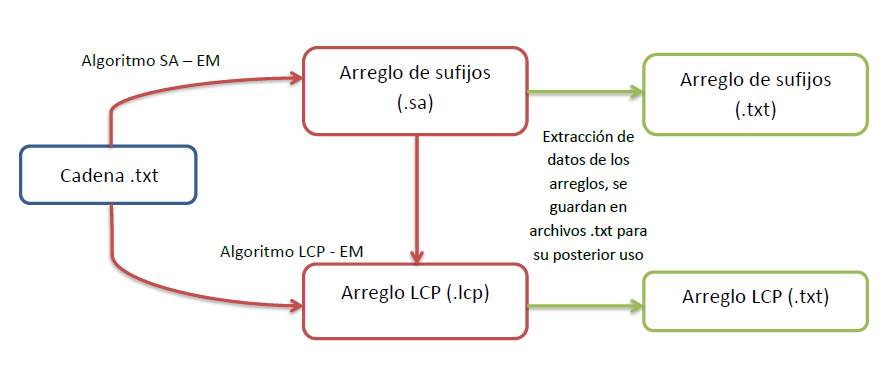
\includegraphics[width=1.0\textwidth]{./images/esquema_v1.PNG}
    \caption{Esquema sencillo de transformación de archivos para usarlos en el programa principal}
    \label{fig:imple1}
\end{figure}

Esto implica un gran uso de disco duro como punto en contra, más aún si se tiene que el archivo ``TrEMBL'' es muy pesado. Por lo tanto los pesos usados según cada archivo son los siguientes:

\begin{table}[h]
\centering
\begin{tabular}{|l|c|c|c|c|c|}
\hline
\multicolumn{1}{|c|}{\textbf{Base de Datos}} & \textbf{Archivo .sa} & \textbf{Archivo .lcp} & \textbf{\begin{tabular}[c]{@{}c@{}}Archivo\\accesible SA\end{tabular}} &  \textbf{\begin{tabular}[c]{@{}c@{}}Archivo\\accesible LCP\end{tabular}} & \textbf{Total}\\ \hline
SwissProt    & 997,5 MB                & 997,5 MB                 & 1,9 GB   & 524,8 MB & 4,41 GB\\
TrEMBL        & 151 GB              & 151 GB       & 351,3 GB   & 85,3 GB & 738,6 GB  \\
EROP-Moscow        & 1,8 MB                 & 1,8 MB                  & 2,4 MB         & 807,9 KB   &  6,80 MB \\
Proteínas humanas     & 191 MB                 & 191 MB                  & 332,6 MB       & 120,8 MB     &  835,4 MB  \\ \hline
\end{tabular}
\caption{Tamaños de archivos guardados en disco duro utilizando ``Algoritmo Memoria Externa''}
\label{tb:labelr15}
\end{table} 

En consecuencia, los tamaños de los datos se hacen poco manejables, en especial con el archivo que guarda los valores del arreglo de sufijos. Ya que \textbf{los elementos que componen un arreglo de sufijos son todos números diferentes} por ende al ir guardando números más grandes el peso requirido se va haciendo más alto; no obstante, el arreglo LCP sí admite valores repetidos.\\
Así pues el usar este algoritmo de memoria externa implica un importante uso de la capacidad del disco duro, sin embargo, en computadores actuales es factible guardar tamaña cantidad de datos, lo cual se mantendría si incluso se desea aumentar la capacidad de memoria RAM disponible para construir los arreglos en memoria externa, descendiendo los tiempos de obtención de estos archivos; aunque es difícil encontrar ordenadores con una memoria RAM superior a 20 GB con excepción de servidores de alta capacidad. 

\subsection{Fragmentos de proteínas de largo entre $k = 1$ hasta $k = 10$}

Los resultados obtenidos tomaron un rango de $k$ que va entre 1 hasta 50. En esta subsección se mostrarán los 10 primeros valores de $k$ (desde 1 hasta 10), ya que son los valores más relevantes con respecto a los péptidos y porcentaje de residuos encontrados. Las tablas completas ($k$ hasta 50) se encuentran en la sección \textbf{Apéndice}.

Siguiendo la ``Tabla 1'' que aparece en \cite{searching} se mostrarán los diferentes substrings encontrados para cada uno de los 4 archivos analizados, comparando según corresponda entre los algoritmos utilizados.

\subsubsection{Base de Datos SwissProt}

Los resultados obtenidos utilizando la base de datos de SwissProt son los siguientes:

\begin{table}[h]
\centering
    \begin{tabular}{| c  r  r  c  r  c |}
    \hline
   \textbf{\begin{tabular}[c]{@{}c@{}}Largo\\péptido ($N$)\end{tabular}} & \multicolumn{1}{c}{\textbf{\begin{tabular}[c]{@{}c@{}}N-péptidos\\posibles ($20^{N}$)\end{tabular}}} & \textbf{\begin{tabular}[c]{@{}c@{}}Encontrados\\``AMI''\end{tabular}} & \textbf{\begin{tabular}[c]{@{}c@{}}Porcentaje\\encontrado (\%)\end{tabular}} & \textbf{\begin{tabular}[c]{@{}c@{}}Encontrados\\``AME''\end{tabular}} & \textbf{\begin{tabular}[c]{@{}c@{}}Porcentaje\\encontrado (\%)\end{tabular}} \\ \hline
    1 & 20 & 20 & 100,00 & 20 & 100,00 \\ \hline
    2 & 400 & 400 & 100,00 & 400 & 100,00 \\ \hline
    3 & 8.000 & 8.000 & 100,00 & 8.000 & 100,00 \\ \hline
    4 & 160.000 & 159.999 & 99,99 & 159.998 & 99,99\\ \hline
    5 & 3.200.000 & 3.113.509 & 97,29 & 3.113.510 & 97,29\\ \hline
    6 & 64.000.000 & 32.921.109 & 51,43 & 32.921.095 & 51,43\\ \hline
    7 & 1.280.000.000 & 84.118.859 & 6,57  & 84.118.817 & 6,57\\ \hline
    8 & 25.600.000.000 & 100.896.814 & 0,39 & 100.896.768 & 0,39\\ \hline
    9 & 512.000.000.000 & 105.834.330 & 0,020  & 105.834.282 & 0,020  \\ \hline
    10 & \multicolumn{1}{c}{1,024$\times 10^{13}$} & 108.976.567 & 0,0010 & 108.976.518 & 0,0010 \\ \hline   
    \end{tabular}
    \caption{Resultados de diferentes substrings obtenidos con la base de datos de SwissProt}
    \label{tb:labelr6}
\end{table}

Es posible identificar que los todos los potenciales residuos hasta un tamaño $k=3$ existen en esta base de datos, consideración importante si se tiene que las proteínas que componen este archivo no superan los 600.000. A partir de allí, a medida que $k$ asciende aparecen más péptidos pero no aumentan al mismo ritmo que los potenciales residuos, por tanto, aparece el brusco descenso de porcentaje, a ello se le agrega que los diferentes substrings encontrados se atascan en los 100 millones de proteínas ($10^{8}$) si $k$ sigue en aumento (ver gráfico \ref{fig:sprot}).

\begin{figure}[h]
    \centering
    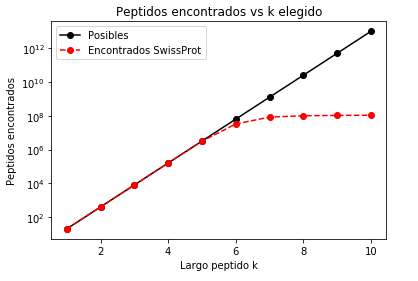
\includegraphics[width=0.6\textwidth]{./images/swissprotv1.png}
    \caption{Gráfico que muestra la cantidad de residuos encontrados según el largo de péptido $k$ para el archivo SwissProt.}
    \label{fig:sprot}
\end{figure}

Con $k=10$ o superior el porcentaje de péptidos diferentes encontrados en relación a los potenciales \textbf{se hace ínfimo}, a niveles millodecimales. Por esta razón que aunque se presenten diferentes valores de residuos encontrados con los 2 algoritmos, si se lleva eso a porcentaje para ambos casos es lo mismo.

En el siguiente gráfico es más fácil identificar el fenómeno de aumento de péptidos en comparación con los potenciales péptidos a encontrar:


\subsubsection{Base de Datos TrEMBL}

Acá solamente se obtuvieron resultados con el ``Algoritmo Memoria Externa'' por las razones explicadas anteriormente, estos resultados son los siguientes:

\begin{table}[h]
\centering
    \begin{tabular}{| c  r  r  c |}
    \hline
   \textbf{\begin{tabular}[c]{@{}c@{}}Largo\\péptido ($N$)\end{tabular}} & \textbf{\begin{tabular}[c]{@{}c@{}}N-péptidos\\posibles ($20^{N}$)\end{tabular}} & \textbf{\begin{tabular}[c]{@{}c@{}}Encontrados\\``AME''\end{tabular}} & \textbf{\begin{tabular}[c]{@{}c@{}}Porcentaje\\encontrado (\%)\end{tabular}} \\ \hline
   
   1 & 20 & 20 & 100,00 \\ \hline
   2 & 400 & 400 & 100,00 \\ \hline
   3 & 8.000 & 8.000 & 100,00 \\ \hline
   4 & 160.000 & 160.000 & 100,00  \\ \hline
   5 & 3.200.000 & 3.200.000 & 100,00  \\ \hline
   6 & 64.000.000 & 63.817.907 & 99,71  \\ \hline
   7 & 1.280.000.000 & 1.024.659.629 & 80,05 \\ \hline
   8 & 25.600.000.000 & 5.743.538.889 & 22,43 \\ \hline
   9 & 512.000.000.000 & 10.114.868.387 & 1,97  \\ \hline
   10 & \multicolumn{1}{c}{1,024$\times 10^{13}$} & 11.524.607.918 & 0,11  \\ \hline
    \end{tabular}
    \caption{Resultados de diferentes substrings obtenidos con la base de datos TrEMBL}
    \label{tb:labelr7}
\end{table}

La base de datos TrEMBL tiene un total de prácticamente 90 millones de proteínas, casi 164 veces el total de proteínas de la base de datos SwissProt. Por lo tanto, es esperable encontrar una mayor cantidad de diferentes residuos y un porcentaje mayor con respecto al universo completo de posibles péptidos a encontrar para determinado $k$. Pues bien, los resultados muestran que esa tendencia se cumple a cabalidad, porque en este archivo \textbf{se encontraron todos los potenciales residuos desde los aminoácidos hasta los pentapéptidos (péptidos compuestos de 5 aminoácidos)}. Con residuos de mayor tamaño ($k=6$ en adelante) comienza a bajar el porcentaje de péptidos encontrados, y sucede el mismo fenómeno que con el archivo SwissProt, los residuos diferentes encontrados se estancan en los 11 mil millones (orden de $10^{10}$) y a pesar que siguen en aumento conforme el valor de $k$ se incrementa, no lleva el mismo ritmo que los potenciales residuos a encontrar, tanto es así que para los péptidos compuestos de 10 aminoácidos los residuos encontrados solamente conforman el 0.1\% del universo total de residuos posibles.

El siguiente gráfico muestra el fenómeno de aumento de péptidos en comparación con los potenciales péptidos a encontrar para la base de datos TrEMBL:

\begin{figure}[h]
    \centering
    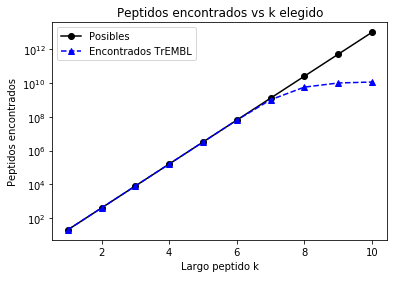
\includegraphics[width=0.6\textwidth]{./images/tremblv1.png}
    \caption{Gráfico que muestra la cantidad de residuos encontrados según el largo de péptido $k$ para el archivo TrEMBL.}
    \label{fig:trembl}
\end{figure}


\subsubsection{Base de Datos EROP-Moscow}

Para esta base de datos los resultados que se obtuvieron con ambos algoritmos son los siguientes:

\begin{table}[h]
\centering
    \begin{tabular}{| c  r  r  c  r  c |}
    \hline
   \textbf{\begin{tabular}[c]{@{}c@{}}Largo\\péptido ($N$)\end{tabular}} & \textbf{\begin{tabular}[c]{@{}c@{}}N-péptidos\\posibles ($20^{N}$)\end{tabular}} & \textbf{\begin{tabular}[c]{@{}c@{}}Encontrados\\``AMI''\end{tabular}} & \textbf{\begin{tabular}[c]{@{}c@{}}Porcentaje\\encontrado (\%)\end{tabular}} & \textbf{\begin{tabular}[c]{@{}c@{}}Encontrados\\``AME''\end{tabular}} & \textbf{\begin{tabular}[c]{@{}c@{}}Porcentaje\\encontrado (\%)\end{tabular}} \\ \hline
    1 & 20 & 20 & 100,00 & 20 & 100,00 \\ \hline
    2 & 400 & 400 & 100,00 & 400 & 100,00 \\ \hline
    3 & 8.000 & 7.907 & 98,83 & 7.907 & 98,83 \\ \hline
    4 & 160.000 & 69.218 & 43,26 & 69.219 & 43,26 \\ \hline
    5 & 3.200.000 & 116.454 & 3,63 & 116.457 & 3,63 \\ \hline 
    \end{tabular}
\end{table}

\newpage
 
\begin{table}[h]
\centering
    \begin{tabular}{| c  r  r  c  r  c |}
    \hline
   \textbf{\begin{tabular}[c]{@{}c@{}}Largo\\péptido ($N$)\end{tabular}} & \textbf{\begin{tabular}[c]{@{}c@{}}N-péptidos\\posibles ($20^{N}$)\end{tabular}} & \textbf{\begin{tabular}[c]{@{}c@{}}Encontrados\\``AMI''\end{tabular}} & \textbf{\begin{tabular}[c]{@{}c@{}}Porcentaje\\encontrado (\%)\end{tabular}} & \textbf{\begin{tabular}[c]{@{}c@{}}Encontrados\\``AME''\end{tabular}} & \textbf{\begin{tabular}[c]{@{}c@{}}Porcentaje\\encontrado (\%)\end{tabular}} \\ \hline
    6 & 64.000.000 & 125.036 & 0,19 & 125.039 & 0,19 \\ \hline
    7 & 1.280.000.000 & 125.750 & 0,0098  & 125.752 & 0,0098 \\ \hline
    8 & 25.600.000.000 & 124.054 & 4,84$\times 10^{-4}$ & 124.055 & 4,84$\times 10^{-4}$\\ \hline
    9 & 512.000.000.000 & 121.103 & 2,36$\times 10^{-5}$  & 121.103 & 2,36$\times 10^{-5}$  \\ \hline
    10 & \multicolumn{1}{c}{1,024$\times 10^{13}$} & 117.457 & 1,14$\times 10^{-6}$ & 117.457 & 1,14$\times 10^{-6}$ \\ \hline   
    \end{tabular}
    \caption{Resultados de diferentes substrings obtenidos con el archivo EROP-Moscow}
    \label{tb:labelr8}
\end{table}

La base de datos EROP-Moscow se compone de 14.785 oligopéptidos cuyos tamaños varían entre 2 a 50 aminoácidos, por lo mismo se hace mucho más complejo encontrar un vasto conjunto de diferentes residuos para cada $k$. No obstante se encuentran \textbf{todos los posibles aminoácidos y dipéptidos existentes}, y con residuos de tamaño $k=3$ en adelante el porcentaje de péptidos encontrados se hace muy pequeño, lo cual es lógico ya que para tal cantidad de péptidos en este archivo es muy difícil obtener una mayor cantidad de diferentes péptidos. Este valor se estanca hasta los 125000 aproximadamente (orden de $10^{5}$ - ver gráfico \ref{fig:erop}), y a partir de los residuos de tamaño $k=8$ el valor disminuye. Una explicación aparente para esto es que existen muchos péptidos compuestos de 5 aminoácidos o menos, por lo mismo para buscar péptidos con una magnitud de más de 5 aminoácidos son pocos los oligopéptidos del conjunto completo que cumplen la condición anteriormente mencionada, que se hace más notoria inclusive aumenta el valor de $k$. Por ejemplo en el caso de la búsqueda de residuos de tamaño $k=50$ se obtuvieron 116 elementos, que son 116 péptidos compuestos de 50 aminoácidos encontrados en la base de datos de EROP-Moscow sin elementos prohibidos.

\begin{figure}[!htb]
    \centering
    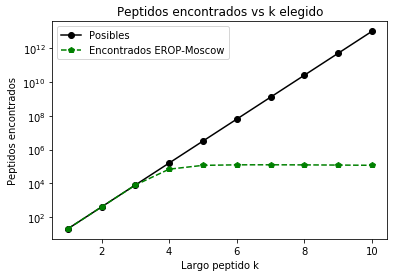
\includegraphics[width=0.6\textwidth]{./images/eropv1.png}
    \caption{Gráfico que muestra la cantidad de residuos encontrados según el largo de péptido $k$ para el archivo EROP-Moscow.}
    \label{fig:erop}
\end{figure}


\subsubsection{Proteínas Humanas}

Para este archivo solo se obtuvieron los diferentes substrings para $k=1$ y los resultados son los siguientes:

\begin{table}[h]
\centering
    \begin{tabular}{| c  c  c  c  c  c |}
    \hline
   \textbf{\begin{tabular}[c]{@{}c@{}}Largo\\péptido ($N$)\end{tabular}} & \textbf{\begin{tabular}[c]{@{}c@{}}N-péptidos\\posibles ($20^{N}$)\end{tabular}} & \textbf{\begin{tabular}[c]{@{}c@{}}Encontrados\\``AMI''\end{tabular}} & \textbf{\begin{tabular}[c]{@{}c@{}}Porcentaje\\encontrado (\%)\end{tabular}} & \textbf{\begin{tabular}[c]{@{}c@{}}Encontrados\\``AME''\end{tabular}} & \textbf{\begin{tabular}[c]{@{}c@{}}Porcentaje\\encontrado (\%)\end{tabular}} \\ \hline
    1 & 20 & 20 & 100,00 & 20 & 100,00 \\ \hline  
    \end{tabular}
    \caption{Resultados de diferentes substrings obtenidos con el archivo Proteínas Humanas}
    \label{tb:labelr9}
\end{table}

En lo que corresponde a las proteínas que existen en el ser humano se puede rescatar que utilizando ambos algoritmos \textbf{se obtienen los 20 aminoácidos buscados (100\%)}. Como para este archivo se está trabajando con solo un $k=1$, se realizará un mayor análisis biológico en la subsección siguiente, para este caso, aquellos aminoácidos que más se repiten.

De igual manera se mostrará el gráfico generado para este archivo:

\begin{figure}[!htb]
    \centering
    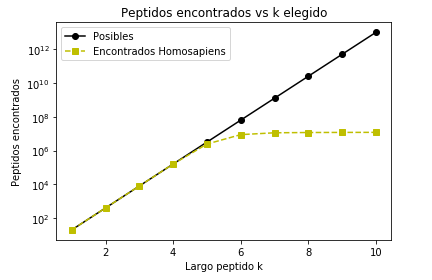
\includegraphics[width=0.6\textwidth]{./images/hsv1.png}
    \caption{Gráfico que muestra la cantidad de residuos encontrados según el largo de péptido $k$ para el archivo Homosapiens.}
    \label{fig:hs}
\end{figure}

\subsubsection{Diferencias entre resultados obtenidos utilizando el ``Algoritmo Memoria Interna'' y el ``Algoritmo Memoria Externa''}

En las tablas mostradas anteriormente, para los archivos SwissProt y EROP-Moscow se identifica que según un determinado $k$ varios de los diferentes substrings encontrados entrega diferentes valores usando ambos algoritmos ($k=4$ o superior para base de datos SwissProt y varios $k$ para EROP-Moscow). ¿Esto implica que uno de los algoritmos utilizados está incorrecto? ¿O acaso los 2 algoritmos están incorrectos?\\
Cuando se comenzó a trabajar con este tipo de cadenas, destacados investigadores como Gonzalo Navarro \cite{navarro2016} han expuesto que utilizar datos compactos es lo más conveniente, porque el procesamiento de texto es más rápido y expedito de comprender. Dentro de esto grupo enorme de estructuras que trabajan con datos tipo cadena se eligió el arreglo de sufijos y el arreglo LCP.\\
Pues bien, para llevar a tierra todo lo investigado en información es importante obtener \textbf{datos concretos de experimentación}, que se han mostrado en cada uno de los Tablas anteriores. Por consiguiente al experimentar con estos algoritmos es bastante factible obtener varias diferencias de resultados obtenidos, que según apreciando el porcentaje de péptidos encontrados, son los mismos, a tal punto que se necesita \textbf{llegar a la tercera o cuarta cifra significativa para recíen encontrar diferencias} entre estos porcentajes.

Observando desde el lado de la implementación realizada, los arreglos obtenidos se aplican según esquemas establecidos por investigadores, para el lado del algoritmo desarrollado por Kasai \cite{kasai} como para los algoritmos de memoria externa (\cite{sascan}, \cite{emsparse}), por ende se hallan diferencias de implementación los cuales definan estas diferencias de resultados. Otra cosa importante es que las cadenas usadas son tan grandes que ocupan tamaños cercanos a los 200 millones de caracteres, a los cuales se le revisa su posición y sufijo al que pertenece para poder extraer aquel residuo con su número (cantidad de veces que aparece en la base de datos) y guardarlo en el \textit{priority queue}, por ende el procedimiento realizado también puede dar con estas diferencias que a la larga son muy pequeñas por los porcentajes que se obtuvieron.

Para intentar corroborar se podría usar una opción poco ortodoxa, que sería obtener los diferentes substrings para cada archivo usando un algoritmo de fuerza bruta, pero realizar esto no es recomendable ya que a nivel de tiempo es el algoritmo más malo que se puede hallar, si se entrega como \textit{input} el archivo de TrEMBL a este algoritmo demoraría meses en obtener los resultados solicitados.

Los péptidos encontrados para cada archivo según el largo $k$ del péptido se adjuntan en el siguiente gráfico:

\begin{figure}[h]
    \centering
    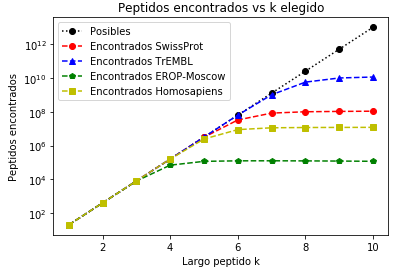
\includegraphics[width=0.6\textwidth]{./images/todosv1.png}
    \caption{Gráfico que muestra los residuos encontrados según el largo de péptido $k$ para los 4 archivos.}
    \label{fig:todos}
\end{figure}

Tomando en consideración esto, se procederá a resumir en un gráfico de Porcentaje v/s $k$ cómo evoluciona el porcentajes de péptidos encontrados según los péptidos posibles a encontrar:

\begin{figure}[h]
    \centering
    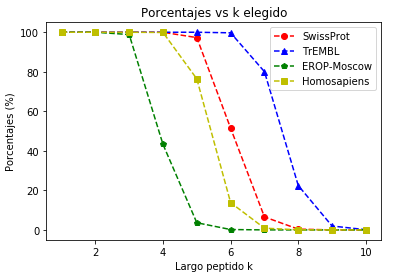
\includegraphics[width=0.6\textwidth]{./images/grafico1v1.png}
    \caption{Porcentajes de péptidos encontrados según el largo de péptido $k$ para los 4 archivos.}
    \label{fig:imple2}
\end{figure}

Observando el gráfico (Figura \ref{fig:imple2}), se aprecia que los valores obtenidos en los porcentajes dependen \textbf{directamente de la cantidad de proteínas} que contenga la base de datos (la relación de tamaños de los archivos sigue el siguiente patrón: TrEMBL $>$ SwissProt $>$ Homosapiens $>$ EROP-Moscow), es decir, si se tienen más proteínas será mayor la diversidad de residuos a encontrar. Hasta $k=3$ es posible identificar en todos los archivos que poseen casi todos los residuos posibles, a partir de ese punto comienzan a bajar los porcentajes de fragmentos encontrados de tamaño $k$. En todos los casos esta bajada en porcentajes es brusca, tomando en cuenta que los posibles péptidos de tamaño $k$ se rigen según la fórmula $20^{k}$. Al contener esta fórmula como base al 20, el salto exponencial que implica ir de $k$ a $k+1$ es muy fuerte, tanto es así que por ejemplo el archivo TrEMBL, a pesar de ser 164 veces más grande que el archivo SwissProt, abarca solamente un 20\% de los posibles residuos que se pueden encontrar de tamaño 8 ($20^{8} = 25.600.000.000$), mientras que SwissProt abarca menos del 0.5\% de residuos posibles para este $k$.\\
Para $k=10$ los porcentajes de péptidos encontrados para los 4 archivos es prácticamente 0, por esa razón es que se decidió mostrar los el comportamiento de los diferentes substrings localizados hasta un tamaño igual a 10, para $k$ mayores a este valor los resultados de los porcentajes serían muy pequeños, prácticamente a escalas atómicas. 

\subsection{Fragmentos de proteínas de determinado $k$ que más se repiten}

Ahora se mostrarán los substrings de tamaño $k$ que más se repiten en los 4 \textit{datasets} trabajados. Para cada $k$ se obtuvieron los 20 residuos que más se repiten, no obstante por motivos de espacio se mostrarán en esta sección los 5 substrings que más se repiten variando $k$ entre 1 hasta 10 (hasta 8 para SwissProt por motivos de espacios) como se hizo en el análisis anterior (las tablas completas con los 3 substrings que más se repiten variando $k$ entre 1 hasta 50 serán colocadas en la sección \textbf{Apéndice}, se consideraron los 3 primeros por motivos de espacio). Primero se presentarán las tablas obtenidas y luego se le hará un análisis a estos resultados.

\subsubsection{Base de Datos SwissProt}

\begin{table}[h]
\centering
\begin{tabular}{|c|r|r|c|c|r|r|}
\cline{1-3} \cline{5-7}
\textbf{k} & \multicolumn{1}{c|}{\textbf{\begin{tabular}[c]{@{}c@{}}Algoritmo \\ Memoria Interna\end{tabular}}}                          & \multicolumn{1}{c|}{\textbf{\begin{tabular}[c]{@{}c@{}}Algoritmo\\ Memoria Externa\end{tabular}}}                              & \multicolumn{1}{l|}{} & \textbf{k} & \multicolumn{1}{c|}{\textbf{\begin{tabular}[c]{@{}c@{}}Algoritmo\\ Memoria Interna\end{tabular}}}                                                        & \multicolumn{1}{c|}{\textbf{\begin{tabular}[c]{@{}c@{}}Algoritmo\\ Memoria Externa\end{tabular}}}                                                           \\ \cline{1-3} \cline{5-7} 
1  & \begin{tabular}[c]{@{}r@{}}L - 19.206.802\\ A - 16.435.230\\ G - 14.086.821\\ V - 13.664.059\\ E - 13.406.543\end{tabular}      & \begin{tabular}[c]{@{}r@{}}L - 19.206.802\\ A - 16.435.229\\ G - 14.086.821\\ V - 13.664.059\\ E - 13.406.543\end{tabular}      &                       & 5  & \begin{tabular}[c]{@{}r@{}}NNNNN - 36.977\\ QQQQQ - 26.232\\ SSSSS - 17.652\\ AAAAA - 17.020\\ EEEEE - 13.572\end{tabular} & \begin{tabular}[c]{@{}r@{}}NNNNN - 36.977\\ QQQQQ - 26.232\\ SSSSS - 17.652\\ AAAAA - 17.020\\ EEEEE - 13.572\end{tabular} \\ \cline{1-3} \cline{5-7} 
2  & \begin{tabular}[c]{@{}r@{}}LL - 1.886.886\\ AA - 1.714.607\\ AL - 1.683.204\\ LA - 1.673.336\\ LS - 1.337.091\end{tabular}      & \begin{tabular}[c]{@{}r@{}}LL - 1.886.886\\ AA - 1.714.607\\ AL - 1.683.204\\ LA - 1.673.336\\ LS - 1.337.091\end{tabular}      &                       & 6  & \begin{tabular}[c]{@{}r@{}}NNNNNN - 31.269\\ QQQQQQ - 20.197\\ SSSSSS - 10.379\\ AAAAAA - 8.392\\ EEEEEE -   8.077\end{tabular}                       & \begin{tabular}[c]{@{}r@{}}NNNNNN - 31.269\\ QQQQQQ - 20.197\\ SSSSSS - 10.379\\ AAAAAA -   8.392\\ EEEEEE -   8.077\end{tabular}                                     \\ \cline{1-3} \cline{5-7} 
3 & \begin{tabular}[c]{@{}r@{}}AAA - 232.439\\ ALA - 185.750\\ LLL - 180.299\\ LAA - 179.704\\ AAL - 177.751\end{tabular}      & \begin{tabular}[c]{@{}r@{}}AAA - 232.439\\ ALA - 185.750\\ LLL - 180.299\\ LAA - 179.704\\ AAL - 177.751\end{tabular}      &                       & 7  & \begin{tabular}[c]{@{}r@{}}NNNNNNN - 27.091\\ QQQQQQQ - 16.272\\ SSSSSSS -   6.927\\ EEEEEEE -   5.342\\ AAAAAAA -   4.966\end{tabular}                 & \begin{tabular}[c]{@{}r@{}}NNNNNNN - 27.091\\ QQQQQQQ - 16.272\\ SSSSSSS -   6.927\\ EEEEEEE -   5.342\\ AAAAAAA -   4.966\end{tabular}              \\ \cline{1-3} \cline{5-7} 
4   & \begin{tabular}[c]{@{}r@{}}AAAA - 47.284\\ NNNN - 46.321\\ SSSS - 39.923\\ QQQQ - 36.956\\ EEEE - 29.213\end{tabular}      & \begin{tabular}[c]{@{}r@{}}AAAA - 47.284\\ NNNN - 46.321\\ SSSS - 39.923\\ QQQQ - 36.956\\ EEEE - 29.213\end{tabular}      &                       & 8 & \begin{tabular}[c]{@{}r@{}}NNNNNNNN - 23.879\\ QQQQQQQQ - 13.508\\ SSSSSSSS -   5.006\\ SDSDSDSD -   3.905\\ DSDSDSDS -   3.875\end{tabular}            & \begin{tabular}[c]{@{}r@{}}NNNNNNNN - 23.879\\ QQQQQQQQ - 13.508\\ SSSSSSSS -   5.006\\ SDSDSDSD -   3.905\\ DSDSDSDS -   3.875\end{tabular}       \\ \cline{1-3} \cline{5-7} 
\end{tabular}
\caption{Residuos más repetidos usando $k$ entre 1 hasta 8 para la base de datos SwissProt.}
\label{tb:labelr10}
\end{table}

Apreciando bien se identifica que para los 2 algoritmos los resultados obtenidos son los mismos. Por otra parte, las repeticiones van disminuyendo muy rápidamente (para $k = 1$ los valores repetidos superan las 10 millones de repeticiones y para $k = 2$ rondan solamente el millón de repeticiones). Otro punto relevante es que muchas repeticiones son residuos compuestos solamente por un aminoácido.

\newpage

\subsubsection{Base de Datos TrEMBL}

\begin{table}[h]
\centering
\begin{tabular}{|c|r|c|c|r|}
\cline{1-2} \cline{4-5}
\textbf{k} & \multicolumn{1}{c|}{\textbf{\begin{tabular}[c]{@{}c@{}}Algoritmo\\ Memoria Externa\end{tabular}}}   & \multicolumn{1}{l|}{} & \textbf{k} & \multicolumn{1}{c|}{\textbf{\begin{tabular}[c]{@{}c@{}}Algoritmo\\ Memoria Externa\end{tabular}}}   \\ \cline{1-2} \cline{4-5} 
1  & \begin{tabular}[c]{@{}r@{}}L - 2.966.351.173\\ A - 2.715.689.443\\ G - 2.175.272.504\\ V - 2.065.665.475\\ S - 2.030.276.782\end{tabular} &  & 6  & \begin{tabular}[c]{@{}r@{}}QQQQQQ - 2.355.101\\ AAAAAA - 1.496.140\\ SSSSSS - 1.411.002\\ GGGGGG - 898.024\\ NNNNNN - 861.564\end{tabular}                        \\ \cline{1-2} \cline{4-5} 
2  & \begin{tabular}[c]{@{}r@{}}AA - 313.028.096\\ LL - 306.619.288\\ LA - 285.314.569\\ AL - 281.904.750\\ AG - 212.968.976\end{tabular}       &                       & 7  & \begin{tabular}[c]{@{}r@{}}QQQQQQQ - 1.798.936\\ SSSSSSS - 922.266\\ AAAAAAA - 880.843\\ WTVYPPL - 815.253\\ GWTVYPP - 814.768\end{tabular}             \\ \cline{1-2} \cline{4-5}  
3 & \begin{tabular}[c]{@{}r@{}}AAA - 45.269.369\\ LAA - 34.321.839\\ ALA - 34.225.481\\ AAL - 33.850.558\\ LLL - 32.856.884\end{tabular}     &                       & 8 & \begin{tabular}[c]{@{}r@{}}QQQQQQQQ - 1.408.675\\ GWTVYPPL - 813.630\\ TGWTVYPP - 798.282\\ GTGWTVYP - 798.215\\ MIFFMVMP - 771.616\end{tabular}            \\ \cline{1-2} \cline{4-5} 
4   & \begin{tabular}[c]{@{}r@{}}AAAA - 9.197.193\\ SSSS - 5.754.913\\ ALAA - 5.176.104\\ LLLL - 5.111.818\\ AALA - 5.085.892\end{tabular}   &                       & 9  & \begin{tabular}[c]{@{}r@{}}QQQQQQQQQ - 1.124.827\\ GTGWTVYPP - 797.778\\ TGWTVYPPL - 797.178\\ LLLLSLPVL - 756.549\\ LLLSLPVLA - 751.235\end{tabular}      \\ \cline{1-2} \cline{4-5} 
5  & \begin{tabular}[c]{@{}r@{}}QQQQQ - 3.210.070\\ AAAAA - 3.108.174\\ SSSSS - 2.473.516\\ GGGGG - 1.679.232\\ PPPPP - 1.473.476\end{tabular} &                       & 10 & \begin{tabular}[c]{@{}r@{}}QQQQQQQQQQ - 911.438\\ GTGWTVYPPL - 796.679\\ LLLLSLPVLA - 749.816\\ PDMAFPRMNN - 667.479\\ FPRMNNMSFW - 661.041\end{tabular}  \\ \cline{1-2} \cline{4-5} 
\end{tabular}
\caption{Residuos más repetidos usando $k$ entre 1 hasta 10 para la base de datos TrEMBL}
\label{tb:labelr11}
\end{table}

Acá solo se muestran los resultados con los algoritmos de memoria externa ya que con el Algoritmo Memoria Interna no se pudo analizar esta base de datos (los motivos fueron explicados anteriormente).\\
Los péptidos más repetidos obtenidos para esta base de datos entregan resultados muy similares a los conseguidos con la base de datos SwissProt con respecto a \textbf{los residuos}. Este fenómeno será explicado más adelante.

\newpage

\subsubsection{Base de Datos EROP-Moscow}

\begin{table}[h]
\centering
\begin{tabular}{|c|r|r|c|c|r|r|}
\cline{1-3} \cline{5-7}
\textbf{k} & \multicolumn{1}{c|}{\textbf{\begin{tabular}[c]{@{}c@{}}Algoritmo \\ Memoria Interna\end{tabular}}}                & \multicolumn{1}{c|}{\textbf{\begin{tabular}[c]{@{}c@{}}Algoritmo\\ Memoria Externa\end{tabular}}}                    & \multicolumn{1}{l|}{} & \textbf{k} & \multicolumn{1}{c|}{\textbf{\begin{tabular}[c]{@{}c@{}}Algoritmo\\ Memoria Interna\end{tabular}}}                                     & \multicolumn{1}{c|}{\textbf{\begin{tabular}[c]{@{}c@{}}Algoritmo\\ Memoria Externa\end{tabular}}}                                        \\ \cline{1-3} \cline{5-7} 
1                                                                      & \begin{tabular}[c]{@{}r@{}}G - 30.373\\ L - 23.867\\ K - 21.956\\ S - 21.486\\ C - 21.365\end{tabular}           & \begin{tabular}[c]{@{}r@{}}G - 30.373\\ L - 23.867\\ K - 21.956\\ S - 21.486\\ C - 21.365\end{tabular}           &                       & 6                                                                      & \begin{tabular}[c]{@{}r@{}}RRRRRR - 160\\ FDEIDR - 127\\ NFDEID - 114\\ CGLSGL - 98\\ GLSGLC - 94\end{tabular}                  & \begin{tabular}[c]{@{}r@{}}RRRRRR - 160\\ FDEIDR - 127\\ NFDEID - 114\\ CGLSGL - 98\\ GLSGLC - 94\end{tabular}                  \\ \cline{1-3} \cline{5-7} 
2                                                                      & \begin{tabular}[c]{@{}r@{}}GL - 3.307\\ RR - 2.904\\ GG - 2.872\\ GK - 2.558\\ AA - 2.493\end{tabular}           & \begin{tabular}[c]{@{}r@{}}GL - 3.307\\ RR - 2.904\\ GG - 2.872\\ GK - 2.558\\ AA - 2.493\end{tabular}           &                       & 7                                                                      & \begin{tabular}[c]{@{}r@{}}NFDEIDR - 102\\ CGLSGLC - 88\\ VCGLSGL - 79\\ MEHFRWG - 76\\ FDEIDRS - 72\end{tabular}               & \begin{tabular}[c]{@{}r@{}}NFDEIDR - 102\\ CGLSGLC - 88\\ VCGLSGL - 79\\ MEHFRWG - 76\\ FDEIDRS - 72\end{tabular}               \\ \cline{1-3} \cline{5-7} 
3                                                                      & \begin{tabular}[c]{@{}r@{}}RRR - 1.253\\ FGL - 483\\ GGG - 479\\ LSG - 469\\ AAK - 451\end{tabular}          & \begin{tabular}[c]{@{}r@{}}RRR - 1.253\\ FGL - 483\\ GGG - 479\\ LSG - 469\\ AAK - 451\end{tabular}          &                       & 8                                                                      & \begin{tabular}[c]{@{}r@{}}VCGLSGLC - 71\\ EHFRWGKP - 68\\ MEHFRWGK - 68\\ SMEHFRWG - 65\\ YSMEHFRW - 62\end{tabular}           & \begin{tabular}[c]{@{}r@{}}VCGLSGLC - 71\\ EHFRWGKP - 68\\ MEHFRWGK - 68\\ SMEHFRWG - 65\\ YSMEHFRW - 62\end{tabular}           \\ \cline{1-3} \cline{5-7} 
4                                                                      & \begin{tabular}[c]{@{}r@{}}RRRR - 712\\ GGGG - 183\\ GCSC - 172\\ CCSG - 167\\ LSGL - 162\end{tabular}      & \begin{tabular}[c]{@{}r@{}}RRRR - 712\\ GGGG - 183\\ GCSC - 172\\ CCSG - 167\\ LSGL - 162\end{tabular}      &                       & 9                                                                      & \begin{tabular}[c]{@{}r@{}}MEHFRWGKP - 68\\ SMEHFRWGK - 65\\ YSMEHFRWG - 61\\ EHFRWGKPV - 59\\ GGTCNTPGC - 59\end{tabular}      & \begin{tabular}[c]{@{}r@{}}MEHFRWGKP - 68\\ SMEHFRWGK - 65\\ YSMEHFRWG - 61\\ EHFRWGKPV - 59\\ GGTCNTPGC - 59\end{tabular}      \\ \cline{1-3} \cline{5-7} 
5                                                                      & \begin{tabular}[c]{@{}r@{}}RRRRR - 373\\ FDEID - 144\\ DEIDR - 139\\ CGLSG - 128\\ GGGGG - 121\end{tabular} & \begin{tabular}[c]{@{}r@{}}RRRRR - 373\\ FDEID - 144\\ DEIDR - 139\\ CGLSG - 128\\ GGGGG - 121\end{tabular} &                       & 10                                                                     & \begin{tabular}[c]{@{}r@{}}SMEHFRWGKP - 65\\ YSMEHFRWGK - 61\\ MEHFRWGKPV - 59\\ SYSMEHFRWG - 53\\ EHFRWGKPVG - 46\end{tabular} & \begin{tabular}[c]{@{}r@{}}SMEHFRWGKP - 65\\ YSMEHFRWGK - 61\\ MEHFRWGKPV - 59\\ SYSMEHFRWG - 53\\ EHFRWGKPVG - 46\end{tabular} \\ \cline{1-3} \cline{5-7} 
\end{tabular}
\caption{Residuos más repetidos usando $k$ entre 1 hasta 10 para la base de datos EROP-Moscow.}
\label{tb:labelr12}
\end{table}

Con esta base de datos ya es posible obtener los resultados con los 2 algoritmos sin problemas, además se aprecia que los valores obtenidos son los mismos para cada algoritmo utilizado.\\
Para esta base de datos los péptidos obtenidos distan de los encontrados en los archivos anteriores, de hecho no aparecen residuos compuestos por un solo aminoácido (a excepción de ``R'' y ``G''), lo que tiene relación con la \textbf{base de datos utilizada}. Al ser este un análisis más biológico, se tratará más adelante.

\subsubsection{Proteínas Humanas}

\begin{table}[h]
\centering
\begin{tabular}{|c|r|r|}
\cline{1-3}
\textbf{k} & \multicolumn{1}{c|}{\textbf{\begin{tabular}[c]{@{}c@{}}Algoritmo \\ Memoria Interna\end{tabular}}}                & \multicolumn{1}{c|}{\textbf{\begin{tabular}[c]{@{}c@{}}Algoritmo\\ Memoria Externa\end{tabular}}}    \\ \cline{1-3}

1                                                                      & \begin{tabular}[c]{@{}r@{}}L - 3.979.937\\ S - 3.123.633\\ A - 2.631.167\\ E - 2.467.325\\ G - 2.448.081\\ P - 2.336.530\\ T - 2.248.068\\ V - 2.229.816\\ K - 2.082.746\\ R - 2.012.813\\ I - 1.863.090\\ D - 1.723.766\\ Q - 1.715.384\\ F - 1.448.281\\ N - 1.448.115\\ Y - 1.078.310\\ H - 997.696\\ M - 922.926\\ C - 805.709\\ W - 527.194\end{tabular} & \begin{tabular}[c]{@{}r@{}}L - 3.979.937\\ S - 3.123.633\\ A - 2.631.167\\ E - 2.467.325\\ G - 2.448.081\\ P - 2.336.530\\ T - 2.248.068\\ V - 2.229.816\\ K - 2.082.746\\ R - 2.012.813\\ I - 1.863.090\\ D - 1.723.766\\ Q - 1.715.384\\ F - 1.448.281\\ N - 1.448.115\\ Y - 1.078.310\\ H - 997.696\\ M - 922.926\\ C - 805.709\\ W - 527.194\end{tabular}           \\ \cline{1-3}

\end{tabular}
\caption{Residuos más repetidos usando $k = 1$ para Proteínas Humanas}
\label{tb:labelr13}
\end{table}


Al ser solamente $k=1$ a analizar para este archivo (se consideró eso ya que la finalidad era identificar a aquellos aminoácidos que más están presentes en el ser humano) se decide mostrar para ambos algoritmos la cantidad de veces que se repiten cada uno de los 20 aminoácidos.\\
Se puede identificar que los resultados obtenidos utilizando cualquiera de los 2 algoritmos es el mismo, lo cual entrega veracidad a los resultados logrados.

\subsubsection{Análisis de resultados (enfoque algorítmico)}

Los resultados conseguidos con los 2 algoritmos en esta sección son similares, por ende otorgan veracidad a la hora de definir que la estrategia de utilizar arreglos de sufijos y arreglos LCP era la indicada. Más importante aún, queda de manifiesto que la opción de uso de la estructura conocida como \textbf{\textit{priority queue}} es la correcta ya que permite guardar substrings enlazados con su respectivo valor para luego extraer aquellos residuos con más altos valores. Su utilización permitió identificar estos datos importantes y construir estas Tablas de información, por consiguiente, parece ser la opción indicada a la hora de buscar ordenar números, strings u otro tipo de variables siguiendo un orden de jerarquía determinado con anterioridad.

\subsubsection{Análisis de resultados (enfoque biológico)}

Recordando un poco, la estructura de un aminoácido sigue el formato mostrado en la Figura \ref{fig:imple3}:

\begin{figure}[h]
    \centering
    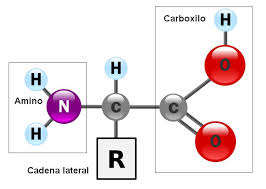
\includegraphics[width=0.4\textwidth]{./images/estructura2.jpeg}
    \caption{Estructura química general de un aminoácido}
    \label{fig:imple3}
\end{figure}

Con respecto a la frecuencia de los residuos de aminoácidos encontrados para la base de datos de UniProt (SwissProt, TrEMBL y Homosapiens), los aminoácidos L (Leucina), A (Alanina), G (Glicina), V (Valina) y E (Ácido Glutámico - aminoácido que posee carga negativa en su grupo radical R) son los más comunes debido a sus características físico-químicas, en especial para L, A y V, que son \textbf{residuos hidrofóbicos} (L es el residuo más hidrofóbico). Cuando se habla de aminoácidos hidrofóbicos \cite{quimicaaminoacidos}, su característica principal es que tienden a rechazar el ambiente acuoso (agua) y, por lo tanto, residen predominante dentro de las proteínas. Estos residuos se utilizan para la estabilización de la estructura global de muchas proteínas (en especial aquellas con más de 50 aminoácidos).\\
Por el contrario, los aminoácidos hidrofílicos tienden a interactuar con el ambiente acuoso, se encuentran ubicados en los sectores extremos de una cadena de polipéptidos y están implicados a menudo en la formación de enlaces de H para la unión entre aminoácidos.

En el caso de los ``oligopéptidos reguladores'' (base de datos de EROP-Moscow) los aminoácidos G, L, K (Lisina - aminoácido que posee carga positiva en su grupo radical R), S (Serina) y C (Cisteína) son los residuos más comunes. Estos oligopéptidos \cite{zamyatnin3} son usualmente moléculas flexibles ya que poseen pocas interacciones intramoleculares débiles, no obstante algunos oligopéptidos tienen enlaces intramoleculares C-C (covalentes) muy fuertes. 

En el caso de ciertos aminoácidos con carga positiva (como el aminoácido K), esta carga positiva en pequeñas moléculas (muchas de ellas contenidas en la base de datos EROP-Moscow) pueden ser muy importantes en la formación de interacciones iónicas (carga con carga) con cargas negativas (como el aminoácido E) de largas moléculas (muchas de ellas que aparecen en la base de datos UniProt).